\chapter{Theory}
\label{chap:theory}
\chapquote{When working toward the solution of a problem, it always helps if you know the answer.}{Rule of Accuracy, from Arthur Bloch's book \textit{Murphy's Law}.}
The standard model of particle physics (SM) is a theory which describes three of the four known fundamental interactions, \ie{}, the strong, the weak and the electromagnetic interaction.
Gravity is not yet included in this theory, but since its coupling is weak w.r.t.\ the other fundamental interactions at scales of particle accelerator energies, the impact can be neglected for all processes within the present analysis.
The standard model uses the framework of a quantum field theory to describe the dynamics of all known fundamental particles.
The description is Lorentz invariant, obeys locality\footnote{The action only contains terms in which the fields and their derivatives are evaluated at the same space-time point.} and probability conservation, and is thus considered a \textit{healthy} theory.
%ensures probability conservation by having unitary Hamiltonians and is thus considered a \textit{healthy} theory.
%Each particle is characterized by a number of \emph{Casimirs}, \ie{} mass and spin, associated with the Poincar\'e group, and charges, associated with internal symmetry groups.

%The standard model is classified as a \emph{healthy} quantum field theory, thus being Lorentz invariant, obeying locality\footnote{The action only contains terms in which the fields and their derivatives are evaluated at the same spacetime point.} and ensuring probability conservation by having unitary Hamilton operators.

The (fundamental) particles are quarks, like the \uquark- and \dquark-quark forming the hadronic matter (\eg{}, protons and neutrons), leptons (\eg{}, electrons and electron neutrinos), and bosons (\eg{}, photons).
Within the SM, these particles are the fundamental excitations of respective fields.
%, \ie{}~do not consist of any sub-structure.

The gauge bosons of this theory arise from Yang-Mills fields.
In total, there are eight massless bosons of the strong interaction (gluons), three massive bosons (\Wpm and \PZ) and one massless boson (photon) of the electro-weak interaction.
One additional boson arises from the Higgs mechanism and brings masses to all fundamental particles which do interact with this boson.
The fundamental fermions of the standard model are arranged in multiplets based on the local symmetries given by the respective Yang-Mills theory:
\begin{align*}
  \ell^i_L &= (\mathbf{1}, \mathbf{2})_{-1} & i &= 1,2,3 \,,\\ 
%  \nu_R &= (\mathbf{1}, \mathbf{1})_0 & \nu &= \nu_e, \nu_\mu, \nu_\tau \,,\\ 
  \ell^i_R &= (\mathbf{1}, \mathbf{1})_{-2} & i &= e^-,\mu^-,\tau^- \,,\\ 
  q^i_L &= (\mathbf{3}, \mathbf{2})_{\frac{1}{3}} & i &= 1,2,3 \,,\\
  u_R &= (\mathbf{3}, \mathbf{1})_{\frac{4}{3}} & u &= u,c,t \,,\\
  d'_R &= (\mathbf{3}, \mathbf{1})_{-\frac{2}{3}} & d &= d,s,b \,,
\end{align*}
where the subscripts $L$ and $R$ indicate whether the particle is left ($L$) or right ($R$) handed, and the bold faced numbers are the representation of the gauge group of the strong interaction and the weak isospin, respectively.
The lower number indicates the weak hypercharge.
The electric charge $q$ of each particle can be determined by the Gell-Mann-Nishijima formula \cite{Nishijima1955,GellMann1956}, yielding a charge of $q = 2/3 \, |e|$ for the up-type quarks \uquark, \cquark, \tquark and $q = -1/3 |e|$ for the down-type quarks $\dquark'$, $\squark'$, $\bquark'$.
The leptons \en, \mun and \taum are charged equally with $q=-|e|$, whereas the neutrinos are neutral and therefore do not couple electro-magnetically.  
Every fermion comes with one anti-fermion.
From a group theoretical point of view, these particles originate from the conjugated fermion representation, whereas from a field theoretical point of view they are obtained by mirroring the charge ($C$) and the parity ($P$) of the respective fermion.

In total, there are six left- and three right-handed leptons, where the former are arranged in weak isospin doublets, \ie{}, $(e_L^-, \nu_e)$, $(\mu_L^-, \nu_\mu)$ and $(\tau_L^-, \nu_\tau)$ and the latter appear in singlets $(e_R^-)$, $(\mu_R^-)$, $(\tau_R^-)$.
%Right handed neutrinos transforms as singlets within the strong interaction as well and, since having a vanishing weak hypercharge, do not interact electro-magnetically.
%herefore they are consider to be \textit{sterile}. 

The six known quarks $\uquark$, $\cquark$, $\tquark$, $\dquark'$, $\squark'$, $\bquark'$ also appear left and right handed.
Again, the latter appears in weak iso-singlets, whereas the former are arranged in weak iso-doublets, \ie{}, $(\uquark,\dquark')$, $(\cquark,\squark')$ and $(\tquark,\bquark')$.
The weak interaction describes the transitions of the left-handed up-type quarks $(\uquark,\cquark,\tquark)$ to the left-handed down-type quarks $(\dquark',\squark',\bquark')$.
This conversion within the weak iso-doublets is mediated via the coupling between the \Wpm bosons and the charged weak current
\begin{equation*}
  \mathscr{J}_\mu^{\text{CC}} = (\uquarkbar, \cquarkbar, \tquarkbar) \, \gamma_\mu \left(1-\gamma_5 \right) \! \begin{pmatrix} \dquark' \\ \squark' \\ \bquark' \end{pmatrix}.
\end{equation*}
In the next section we will elaborate that $(\dquark',\squark',\bquark')$ are the weak flavor eigenstates and differ from the mass eigenstates of the quarks.
Taking this into account leads to the introduction of an unitary matrix that connects flavor and mass eigenstates.
This matrix is called the \gls{ckm} matrix and brings four additional degrees of freedom, \ie{}, three mixing angles and one \CP violating phase.

The gauge groups are described within the framework of semisimple Lie algebras such that the total gauge symmetry of the standard model is:
\begin{equation*}
  \mathscr{F} = \grpsuthree \times \grpsutw \times \grpuone \,,
\end{equation*}
where \grpsuthree is the gauge group of the strong interaction and $\grpsutw \times \grpuone$ is the respective gauge group of the electro-weak interaction.
The Higgs mechanism (spontaneously) breaks this symmetry down to
\begin{equation*}
  \mathscr{F} = \grpsuthree \times \grpsutw \times \grpuone \; \xmapsto{\text{Higgs}} \; \grpsuthree \times \grpuone_\text{em} \,.
\end{equation*}

The Lagrangian of the standard model reads:
\begin{equation*}
  \mathscr{L} = -\frac{1}{2} \operatorname{tr} \left( \mathbf{F}_{\mu\nu} \, \mathbf{F}^{\mu\nu} \right) \\
  + \overline{\psi} \mathrm{i} \slashed{\mathbf{D}} \psi + \mathscr{L}_\text{Yuk} + \left( \mathbf{D}_\mu \, \phi \right)^2 - V(\phi) \,,
\end{equation*}
where we abbreviated 
\begin{equation*}
  \mathbf{F}_{\mu\nu} \, \mathbf{F}^{\mu\nu} = \mathbf{G}_{\mu\nu} \, \mathbf{G}^{\mu\nu} + \mathbf{W}_{\mu\nu} \, \mathbf{W}^{\mu\nu} + \frac{1}{2} \mathbf{B}_{\mu\nu} \, \mathbf{B}^{\mu\nu}
\end{equation*}
and introduced the covariant derivative
\begin{equation*}
  \mathbf{D}_\mu \, \psi = \left( \partial_\mu + \mathrm{i} g_s \mathbf{G}_\mu + \mathrm{i} g \mathbf{W}_\mu + \mathrm{i} g' \mathbf{B}_\mu \right) \psi \,.
\end{equation*}
All fermions fields are gathered in $\psi$, whereas $\phi$ is the Higgs field, coupling left and right handed fermions via a Yukawa coupling $\mathscr{L}_\text{Yuk}$ with an according potential $V(\phi)$.
The tensors $\mathbf{G}_{\mu\nu}$, $\mathbf{W}_{\mu\nu}$ and $\mathbf{B}_{\mu\nu}$ are the field-strength tensors of the gauge bosons.
The former tensor corresponds to the strong interaction, whereas the latter tensors correspond to the electro-weak interaction.
All three tensors are functions of the corresponding gauge fields and of the generator of their gauge groups, \eg{},
\begin{align*}
  \mathbf{G}_{\mu\nu} &= \partial_\mu \mathbf{G}_\nu - \partial_\nu \mathbf{G}_\mu + \mathrm{i} g_s \left[ \mathbf{G}_\mu,\,\mathbf{G}_\nu \right] \nonumber \\
  &= \left( \partial_\mu G^a_\nu - \partial_\nu G^a_\mu - g_s f_{abc} \, G_\mu^b G_\nu^c \right) \frac{\bm{\lambda}_a}{2} \,,
\end{align*}
where $G_\mu^a$ are the gluon fields (index $a$ takes values $1\ldots8$), $f_{abc}$ is the structure constant and $\bm{\lambda}_a$ are the generator of the $\mathrm{SU}(3)$ group.
%(We use the tensor product $\otimes$ to unfold the acting on the spinor space and the corresponding generator space, respectively.)
The fields $G_\mu^a$ are chosen such that the transformation of the field strength tensor is:
\begin{equation*}
  \mathbf{G}_{\mu\nu}(x) \; \xmapsto{\mathrm{SU}(3)} \; \mathbf{U}(x) \, \mathbf{G}_{\mu\nu}(x) \, \mathbf{U}^\dagger(x) \,,
\end{equation*}
with $\mathbf{U}(x) \equiv U(x)$ being an arbitrary transformation of \grpsuthree, thus leaving the total Lagrangian invariant.
We note that applying the trace operation to $\mathbf{G}_\mu \equiv \mathbf{G}_\mu^\dagger = G^a_\mu(x) \, \frac{\bm{\lambda}_a}{2}$ only affects the generator space
\begin{equation*}
  \operatorname{tr} \mathbf{G}_\mu \equiv G^a_\mu(x) \, \operatorname{tr} \frac{\bm{\lambda}_a}{2} \,,
\end{equation*}
thus yielding
\begin{equation*}
  \operatorname{tr} \left( \mathbf{G}_{\mu\nu} \, \mathbf{G}^{\mu\nu} \right) = G_{\mu\nu}^a \, G_b^{\mu\nu} \, \operatorname{tr} \frac{\bm{\lambda}_a \bm{\lambda}_b}{4} = 
  %G_{\mu\nu}^a \, G_b^{\mu\nu} \, \frac{\delta_{ab}}{2} = 
  \frac{1}{2} \, G_{\mu\nu}^a \, G_a^{\mu\nu} \,. 
\end{equation*}
The same holds for the electro-weak case where the generators of the electro-weak $\grpsutw \times \grpuone$ group are the weak isospin $\sigma_a/2$ (Pauli matrices) and the weak hypercharge $Y$.

While the gauge symmetry of the strong interaction is unbroken and all gluons are indistinguishable, the electro-weak sector of the standard model is broken and the respective field excitations become distinguishable.
The physical fields are the charge eigenstates $\mathbf{W}^+_\mu$, $\mathbf{W}^-_\mu$, $\mathbf{Z}_\mu$, and the photon field $\mathbf{A}_\mu$.
They are obtained via the transformations
\begin{align*}
  \mathbf{W}_\mu^\pm &= \mathbf{W}_\mu^1 \pm \mathrm{i} \mathbf{W}_\mu^2 \,, \\ 
  \begin{pmatrix} \mathbf{Z}_\mu \\ \mathbf{A}_\mu \end{pmatrix} &= \begin{pmatrix} \cos \vartheta_W & -\sin \vartheta_W \\ \sin \vartheta_W & \phantom{-} \cos \vartheta_W \end{pmatrix} \begin{pmatrix} \mathbf{W}^3_\mu \\ \mathbf{B}_\mu \end{pmatrix}.
\end{align*}
This coupling also affects their coupling constants $g$ and $g'$, hence it is sensible to introduce the weak mixing angle~$\vartheta_W$ as
\begin{equation*}
  e = g \sin \vartheta_W = \frac{gg'}{\sqrt{g^2 + g'^2}} \,,
\end{equation*}
where $e$ is the electric charge.
With this, the (classical\footnote{Without neutrino masses.}) standard model of particle physics has 18 free parameters in total,
\begin{itemize}[itemsep=2pt,parsep=2pt]
  \item 3 couplings: $g_s$, $e$, $\sin \vartheta_w$,
  \item 2 boson masses: $m_W$, $m_H$,
  \item 3 lepton masses: $m_e$, $m_\mu$, $m_\tau$,
  \item 6 quark masses: $m_u$, $m_d$, $m_s$, $m_c$, $m_t$, $m_b$,
  \item 4 parameters of the \gls{ckm} matrix.
\end{itemize}

For the sake of completeness we note that we did not account for any affects from renormalization in the Lagrangians shown above, although the standard model is a renormalizable theory.
Renormalization changes the behavior of charges and couplings and make these quantities effectively momentum dependent.
When doing actual calculations it is mandatory to take this into account, not least because of observable properties such as the running of coupling constants.
However, the topic of renomoralization is complex and will neither significantly enrich this brief overview substantively, nor yield deeper insights into the presented analysis.

\section{\texorpdfstring{\CP}{CP} Violation}
Above, we have seen that the charged current $\mathscr{J}_\mu^{\text{CC}}$ couples the weak eigenstates.
This coupling is diagonal such that there is no mixing of the eigenstates.
The flavor eigenstates, however, do not correspond to the mass eigenstates, but there is one arbitrary rotation between flavor and mass eigenstates of the up-type quarks and the down-type quarks each.
These two rotations cancel for all terms of the Lagrangian, except for the charged current $\mathscr{J}_\mu^{\text{CC}}$, since this is the only term connecting up- and down-type quarks.
In $\mathscr{J}_\mu^{\text{CC}}$ both rotations appear in product, thus collapsing to one unitary matrix $V$:
\begin{equation*}
  \mathscr{J}_\mu^{\text{CC}} = (\overline{\uquark'}, \overline{\cquark'}, \overline{\tquark'}) \, \gamma_\mu \left(1-\gamma_5 \right) \! \begin{pmatrix} \dquark' \\ \squark' \\ \bquark'  \end{pmatrix} =
  (\uquarkbar, \cquarkbar, \tquarkbar) \, \gamma_\mu \left(1-\gamma_5 \right) V \! \begin{pmatrix} \dquark \\ \squark \\ \bquark \end{pmatrix},
\end{equation*}
where the prime indicates mass eigenstates.

The matrix $V$ is called the \gls{ckm} matrix and was first introduced by Kobayashi and Maskawa~\cite{Kobayashi1973} as an extension of the two-dimensional Cabibbo matrix~\cite{Cabibbo1963}.
The \gls{ckm} matrix is parametrized by three mixing angles and one \CP violating phase.
Conventionally, one multiplies $V$ to the right, thus mixing down-type mass eigenstates.
When referring to mass eigenstates, each up-type quark now decays to a superposition of three down-type quarks:
\begin{equation*}
    \begin{pmatrix} \uquark' \\ \cquark' \\ \tquark' \end{pmatrix} = \begin{pmatrix} \uquark \\ \cquark \\ \tquark \end{pmatrix} \quad \text{but} \quad
    \begin{pmatrix} \dquark' \\ \squark' \\ \bquark' \end{pmatrix} = \begin{pmatrix} \Vud & \Vus & \Vub \\ \Vcd & \Vcs & \Vcb \\ \Vtd & \Vts & \Vtb \end{pmatrix} \! \begin{pmatrix} \dquark \\ \squark \\ \bquark \end{pmatrix}.
\end{equation*}

The probability of finding a down-type quark after the decay of an up-type quark $u_i$ in a specific mass eigenstate $d_j$ is proportional to the square of the respective matrix element $V_{ij}$.
Since these matrix elements are complex they differ from the decay of the respective anti-quarks in a complex phase, \ie{}, the transition $\overline{u}_i \to \overline{d}_j$ is proportional to the square of $V^*_{ij}$.
In the absence of multiple decay channels, this phase is unphysical and vanishes after squaring the matrix element. 
In the case of multiple decay channels, all joining the same final state but bringing different strong phases, this phase yields a physical effect in different real valued decay amplitudes between particles and the respective anti-particles.
This effect is called direct \CP violation.

The \gls{ckm} matrix exhibits a clear hierarchy, often expressed in the \gls{wolfenstein}~\cite{wolfenstein}:
\begin{align*}
    V &= \begin{pmatrix} \Vud & \Vus & \Vub \\ \Vcd & \Vcs & \Vcb \\ \Vtd & \Vts & \Vtb \end{pmatrix} \nonumber \\
    &= \begin{pmatrix} 1-\lambda^2/2 & \lambda & A \lambda^3 (\rho -\mathrm{i} \eta) \\ -\lambda & 1-\lambda^2/2 & A \lambda^2 \\ A \lambda^3 (1- \rho - \mathrm{i} \eta) & - A \lambda^2 & 1 \end{pmatrix} + \mathcal{O}(\lambda^4) \,,
\end{align*}
where the four parameters $(A, \lambda, \rho, \eta)$ are real numbers.
Here, $\lambda \approx 0.23$ is the sine of the Cabibbo angle and plays the role of an expansion parameter, whereas $\eta$ represents the \CP violating phase.
Note, that this representation only assigns complex phases to the matrix elements \Vub and \Vtd.
Expanding the \gls{ckm} matrix in higher orders of $\lambda$, brings additional phases to three other matrix elements.

The \gls{ckm} matrix is unitary, thus yielding twelve distinct complex relations among the matrix elements:
\begin{equation*}
   \left( V V^\dagger \right)_{ij} = \left( V^\dagger V \right)_{ij} = \delta_{ij} \,.
\end{equation*}
Six of these twelve relations ($i \neq j$) can be represented geometrically as triangles in the complex plane, \eg{},
\begin{equation*}
    \Vud \Vubs + \Vcd \Vcbs + \Vtd \Vtbs = 0 \,,
\end{equation*}
where the length of the edges are given by the absolute values of each addend.
The three angles are given by the argument of the ratio of neighboring edges, \ie{},
\begin{align*}
    \alpha &= \arg \left( - \frac{\Vtd \Vtds}{\Vud \Vubs} \right) \approx \arg \left( - \frac{1-\rho-\mathrm{i} \eta}{\rho + \mathrm{i} \eta} \right), \\
    \beta &= \arg \left( - \frac{\Vcd \Vcbs}{\Vtd \Vtbs} \right) \approx \arg \left( - \frac{1}{1-\rho-\mathrm{i} \eta} \right), \\
    \gamma &= \arg \left( - \frac{\Vud \Vubs}{\Vcd \Vcbs} \right) \approx \arg \left( \rho + \mathrm{i} \eta \right).
\end{align*}
The unitary of the \gls{ckm} matrix implies $\alpha + \beta + \gamma = \pi$, as well as equal areas of all triangles.
Any discrepancy of these relations would indicate a non unitary \gls{ckm} matrix and thus corresponding to physics beyond the standard model.
At the time of writing, the \gls{ckm} angle $\gamma$ is among the least well known constraints, therefore, being an excellent probe of new physics~\cite{Browder2008,Ciuchini2011}. 

At this point it seems appropriate to mention, that neutrinos are set massless within in the classical standard model, thus excluding lepton mixing.
Ever since the discovery of neutrino oscillation \cite{Fukuda1998,Ahmad2001,Ahmad2002} we yet know that neutrinos must have finite masses and therefore leptons mix also.
The corresponding mixing matrix is called the PMNS matrix \cite{Maki1962} and allows \CP violation for leptons. (See \eg{}, Ref.~\cite{nucpv} for some exciting results for \CP violation measurements in neutrino oscillations.) 
There are at least two (conflicting) extensions to the classical standard model that explain the finite neutrino masses but since there is no clear preference from experimental data which of these extensions can be excluded, we did not account for them in our previous parameter counting.
Anyhow, finite neutrino masses will not influence the results of the present analysis since we are dealing with pure hadronic states.
%As stated above, neutrino masses are not yet included in the standard model and will not influence the results of the present analysis since we are dealing with pure hadronic states.

Another source of \CP violation could occurs in strong decays.
It is easy to extend the standard model accordingly and this extension is occasionally considered \textit{more natural}.
Experiments show, however, that the strong interaction seems to conserve \CP.
This conservation is not yet fully understood and is known as the \textit{Strong \CP Problem} in literature~\cite{Ciuchini2011,Mannel2007,LHCb_strongCP}, but appears in perfect agreement with all experimental results so far.
Therefore, the only source of \CP violation in the classical standard model are weak decays.

%When considering weak decays, it is important to differentiate between flavor and mass eigenstates.
%In the following we will always use the mass eigenstates of quarks, anyhow, we will suppress the prime notation for convenience.

%\section{Charge Conjugation and Parity Symmetry}
%\begin{itemize}
%    \item CPT theorem
%    \begin{itemize}
%        \item appeared for the first time implicitly: 1951 Schwinger (doi:10.1103/PhysRev.82.914)
%        \item proofs
%        \begin{itemize}
%            \item Kong.Dan.Vid.Sel.Mat.Fys.Med. 28N5 (1954) no.5, 1-17
%            \item \href{https://lccn.loc.gov/56040984}{link}
%            \item Bell, J. S. (1954). (Thesis). Birmingham University.
%        \end{itemize}
%        \item Any Lorentz invariant local QFT with Hermitian Hamiltonian must have CPT symmetry
%    \end{itemize}
%    \item Charge reversal in QED
%    \begin{itemize}
%        \item QED is invariant
%        \item $\psi \to \mathrm{i} (\bar \psi \gamma^0 \gamma^2)^T$
%        \item $\bar \psi \to \mathrm{i} (\gamma^0 \gamma^2 \psi)^T$
%        \item $A^\mu \to -A^\mu$
%    \end{itemize}
%    \item Attention: this does not alter chirality: $\neu_L \to \neub_L$ \ie{} C-symmetry is violated maximal in weak interaction (since weak interaction does not couple with $\neub_L$.)
%\end{itemize}
%
\section{Quark Model}
Quantum Chromodynamics (QCD) is the quantum field description of the strong interaction that enlarges the pool of quantum numbers of the standard model.
All quarks now possess the new quantum number \textit{color} which can take on three different values.
QCD is an unbroken \grpsuthree gauge symmetry, acting on the color quantum number.
The eight generators of this Lie-Algebra induce eight massless gauge bosons, called \textit{gluons}.

QCD is a non-abelian gauge theory, hence gluons are charged and interact with each other.
Similar to Quantum Electrodynamics (QED), there exist quark loops which screen the (color) charge at large distances.
In marked contrast to QED the gauge bosons of QCD carry charge themselves, therefore allowing gluon loops at the same level.
The gluon loops anti-screen and dominate the quark loops, hence QCD becomes stronger at large distances.
This feature of QCD confines quarks and gluons such that none of them can be isolated.
Only states forming color singlets can be observed at large distance scales, \ie{}, the possible combinations of quarks~\quark and anti-quarks~\quarkbar are mesons (\qqbar), baryons (\quark\quark\quark), tetraquarks (\quark\quark\quarkbar\quarkbar) and pentaquarks (\quark\quark\quark\quark\quarkbar), as well as their respective anti-particles.
These combinations are called \textit{hadrons}.
Furthermore, combinations of two gluons forming a color singlet (glueballs) are possible.

The masses of quarks forming a hadron are much lighter than the masses of the respective hadron.
The reason for that can be found in the two different mechanisms providing masses to quarks and to hadrons.
The former originates directly from the spontaneous symmetry breaking by the Higgs mechanism, the latter originates from the energy of quark and gluon condensates of the QCD vacuum.
The QCD vacuum includes virtual \qqbar pairs that also contribute to the absolute mass of the hadron.
In order to distinguish between these and the valence quarks, we call these virtual quarks \textit{sea quarks}.

The quark model of particle physics is a classification scheme for hadrons in terms of their valence quarks.
The quantum numbers of the quarks are added, obeying the rules of spin algebras, such that each hadron is uniquely defined by their sum.
Besides spin, quarks have another charge of a \grpsutw symmetry, \textit{isospin}.
The two lightest quarks \uquark and \dquark are arranged in iso-doublets, all other quarks are iso-singlets.
This quantum number turns out to be useful, since QCD is unbroken in terms of isospin, thus giving rise to a conserved quantity. 
(Different masses and electrical charges break this symmetry in the electro-weak sector of the standard model.)
Adding the isospin of quarks, one finds the isospin of hadrons by analyzing the outer product, \eg{}, combining a \uquark- and \dquark-quark (taken form the $(\uquark,\dquark)$ doublet $\bm{2}$), and a \squark-quark (singlet $\bm{1}$) yields,
\begin{equation*}
    \bm{2} \otimes \bm{2} \otimes \bm{1} = \bm{3} \oplus \bm{1} \,,
\end{equation*}
a triplet and a singlet.
The triplet (isospin $I=1$) consists of the three baryons \Sp (\uquark\uquark\squark), \Sz (\uquark\dquark\squark) and \Sm (\dquark\dquark\squark), the singlet ($I=0$) is the \Lz baryon (\uquark\dquark\squark) where we have given the valence quark contents in parentheses.
Note, that the \Sz and the \Lz have the same valence quark content, but different isospin.
Therefore they are distinguishable.
Another prominent example of an isospin pair is the nucleon, having isospin $I = 1/2$.
%~\cite{Heisenberg1932}
The two states, that differ in their valence quark content but are anyhow indistinguishable in strong interactions, are the proton (\uquark\uquark\dquark) and the neutron (\uquark\dquark\dquark).

Below, we give a short overview over the intermediate particles \Lb, \Xibz, \Lz and \Dz which play a major role in the present analysis.
All figures, even though not explicitly marked, are taken from the Particle Data Group~\cite{pdg}:
%\subsection{The \texorpdfstring{\Lb}{Λb} Baryon}
%\subsection{The \texorpdfstring{\Lz}{Λ} Baryon and its Final States}
%\subsection{The \texorpdfstring{\Dz}{Neutral D} Meson and its Final States}
\begin{description}
    \item[\Lb Baryon] In the quark model, the \Lb baryon is an iso-singlet state, consisting of valence quarks \uquark, \dquark and \bquark. The lightest \Lb baryon has $I(J^P) = 0(1/2^+)$. The mass is measured as
    \begin{equation*}
        m(\Lb) = 5.61960(17)\gevcc,
    \end{equation*}
    thus it is the lightest baryon with one \bquark- or \bquarkbar-quark. Energy conservation does not allow for any strong decays, therefore the \Lb decays weakly which explains its relatively long lifetime $\tau(\Lb)$,
    \begin{equation*}
        \tau(\Lb) = 1.471(9) \,\text{ps},
    \end{equation*}
    corresponding to a narrow natural width of roughly $\hbar / \tau \approx \SI{0.4}{\milli\electron\volt}$. The dominant decay modes are \decay{\Lb}{\Lc\ellm\neulb} and \decay{\Lb}{\Lc\Dsm} with a relative decay rate of $10.3(2.2)\,\%$ and $1.10(0.10)\,\%$, respectively. The decays \decay{\Lb}{\PD\Lz} and \decay{\Lb}{\Dstar\Lz} that we study in the present analysis have not yet been observed.
    \item[\Xibz Baryon] In the quark model the \Xib baryons, \Xibz ($\bquark\squark\uquark$) and \Xibm ($\bquark\squark\dquark$), are the constituents of an iso-doublet with $I(J^P) = 1/2(1/2^+)$. Both resonances were discovered at the \gls{tevatron} collider in the years 2011 and 2007~\cite{Xibzdisc,Xibmdisc1,Xibmdisc2} (more than a quarter of a century after the \Lb discovery~\cite{Lbdisc}). The mass of the \Xibz baryon is measured as 
    \begin{equation*}
        m(\Xibz) = 5.7919(5)\gevcc,
    \end{equation*}
    which makes it $172.5(4)\mevcc$ heavier than the \Lb baryon and thus forbids any strong decays such as \decay{\Xibz}{\Lb\Kzb}. In the framework of heavy quark expansion all weakly decaying charmless \bquark-hadrons have the same lifetime up to corrections at the order $(\lqcd/m_{\bquark})^2$, where \lqcd is the energy scale at which the strong coupling becomes large and $m_{\bquark}$ is the mass of the \bquark-quark~\cite{rtXibztLb_theory}. The measured mean lifetime ratio of the \Xibz and the \Lb hadron, $\tau(\Xibz) / \tau(\Lb) = 1.006(21)$~\cite{fXibzfLb}, confirms this expectation. None of the (weak) decays into the final states \Dz\Lz, \Dstar\Lz, \Dz\Sz or \Dz\Xiz, that we consider as signal or (potential) background contributions in the present analysis, have yet been observed.
    \item[\Lz Baryon] We have discussed the \Lz baryon and its role in the quark model previously. The mass is measured as
    \begin{equation*}
        m(\Lz) = 1.115683(6)\,\gevcc.
    \end{equation*}
    The dominant decay modes of the $I(J^P) = 0(1/2^+)$ baryon are \decay{\Lz}{\proton\pim} and \decay{\Lz}{\neutron\piz} with branching fractions of $63.9(5)\,\%$ and $35.8(5)\,\%$, respectively. Whereas the latter mode is almost impossible to reconstruct at \lhcb, the reconstruction of the former is feasible, albeit with the caveat that due to the long lifetime of the $\PV^0$ particle,
    \begin{equation*}
        \tau(\Lz) = 263.2(20) \,\text{ps},
    \end{equation*}
    most decays will take place outside of the \gls{velo} (\cf{} Chap.~\ref{chap:detector}). 
    \item[\Dz Meson] The \Dz is a $I(J^P) = 1/2(0^-)$ meson, consisting of valence quarks \cquark and \uquarkbar with a mass of
    \begin{equation*}
        m(\Dz) = 1.86483(5)\,\gevcc.
    \end{equation*}
    The \gls{pdg} lists more than 300 measured (weak) decay modes of the \Dz meson which explains its relatively short lifetime (in comparison with other weakly decaying hadrons),
    \begin{equation*}
        \tau(\Dz) = 0.4101(15) \,\text{ps}.
    \end{equation*}
    Modes of particular interest for the present analysis (and at future prospects) are the $\decay{\Dz}{\Ph\Ph'}$ modes, where $\Ph$ and $\Ph'$ refer to pions or kaons, and $\decay{\Dz}{\Kmp\pipm\pip\pim}$ modes. The mode \decay{\Dz}{\Km\pip} (\ie{}, $\Ph=\Km$ and $\Ph'=\pip$) is referred to as the Cabibbo favored mode due to its \decay{\cquark}{\squark\uquark\dquarkbar} transition (proportional to $1-\lambda^2$ in the \gls{wolfenstein}). Similarly, the modes \decay{\Dz}{\Kp\Km} and \decay{\Dz}{\pip\pim} are referred to as Cabibbo suppressed (proportional to $\lambda$) and finally \decay{\Dz}{\Kp\pim} is referred to as the Cabibbo doubly suppressed mode (proportional to $\lambda^2$).
\end{description}

%\section{The \texorpdfstring{\Lb}{Λb} Baryons at \texorpdfstring{$pp$}{pp} collisions}
%\subsection{Total Amount of \texorpdfstring{\Lb}{Λb} Baryons at \lhcb{}}
%\begin{itemize}
%    \item Relative production rate $f_{\Lb} / f_d$
%    \begin{itemize}
%        \item Necessary for prediction of total amount of $\Lb \to \Dz \Lz$ (\Gls{fom})
%        \item Rough estimate is fine, because
%        \begin{itemize}
%            \item Normalization is $\Lb \to \Dz \proton \pim$.
%            Thus, relative production rates cancel in first approximation.
%            \item Prediction of total amount of $\Lb \to \Dz \Lz$ is limited by theory prediction which gives only the order of magnitude.
%        \end{itemize}
%        \item Paper \cite{LHCb_fLbfd2011}
%        \item $L = \SI{1}{\per\femto\barn}$, $\sqrt{s} = \SI{7}{\tera\electron\volt}$
%        \item Measure
%        \begin{equation*}
%            \frac{f_{\Lb}}{f_d}(x) = \underbrace{\mathcal{S}}_{\text{constant scale factor}} \times \underbrace{\mathcal{R}(x)}_{\text{efficiency corrected yield}}
%        \end{equation*}
%        \begin{align}
%            \mathcal{S} &=
%            \frac{\BR \left( \Bdb \to \Dp \pim \right)}{\BR \left( \Lb \to \Lc \pim \right)}
%            \times
%            \frac{\BR \left( \Dp \to \Km \pip \pip \right)}{\BR \left( \Lc \to \proton \Km \pip \right)} \\
%            \mathcal{R} &=
%            \frac{N_{\Lb \to \Lc \pim}(x)}{N_{\Bdb \to \Dp \pim}(x)}
%            \times
%            \frac{\varepsilon_{\Bdb \to \Dp \pim}(x)}{\varepsilon_{\Lb \to \Lc \pim}(x)}
%        \end{align}
%        where $x$ denotes $\pt$ or $\eta$.
%        \begin{itemize}
%            \item $\mathcal{R}(x)$ via: $\Lb \to (\proton \Km \pip)_{\Lc} \pim$, $\Bdb \to (\Km \pip \pip)_{\Dp} \pim$, $\pt=\SIrange{1.5}{40}{\gevc}$, $\eta = \numrange{2}{5}$
%            \item $\mathcal{S}$ via: Scale $\mathcal{R}(x)$ to data from Ref.~\cite{LHCb_bProdFrac_7,LHCb_bProdFrac_13}
%            \begin{itemize}
%                \item $\Lb \to \Lc \mun \neumb \PX$, $\Bb \to \PD \mun \neumb \PX$,
%                where the $\PB$ meson is charged or neutral, and $\PX$ represents possible additional decay products of the $b$ hadron that are not included in the candidate reconstruction.
%                \item Assumptions: near equality of the inclusive semileptonic decay width of all $b$ hadrons
%                \item Extract $f_{\Lb}/f_d$ via: isospin symmetry $f_u = f_d$ @ $f_{\Lb}/(f_u+f_d)$
%            \end{itemize}
%        \end{itemize}
%        \item Results:
%        \begin{align}
%            \frac{f_{\Lb}}{f_d}(\pt) &\propto a + \mathrm{e}^{-b \, p_T} \\
%            \frac{f_{\Lb}}{f_d}(\eta) &\propto c + d \, \eta
%        \end{align}
%        with $a, b, c, d > 0$; thus the relative production rate of the $\Lb$ decreases with increasing (decreasing) values for the transverse momentum (pseudo-rapidity).
%        \item Conservative approximation for average
%        \begin{equation*}
%            \left\langle \frac{f_{\Lb}}{f_d} \right\rangle = \numrange{0.2}{0.6}
%        \end{equation*}
%        This range was chosen such that it covers $\Lb$ baryons in the \lhcb{} acceptance and for energies corresponding to Run 1 and Run 2.
%    \end{itemize}
%\end{itemize}

\section{Strong Isospin}
\label{sec:isospin}
In contrast to the electro-weak interaction that breaks various symmetries by allowing flavor transitions, \QCD appears to be invariant under several symmetries.
These symmetries can be categorized into gauge symmetries, \eg{}, color \grpsuthree, accidental symmetries, such as the baryon number conservation, and approximate symmetries.
The (strong) isospin is an approximate symmetry of the SM, but can be considered a conserved symmetry for \QCD.
%In the framework of isospin, the two lightest quarks \uquark and \dquark are arranged within an iso-doublet, all other quarks are (strong) iso-singlets.
%By doing so, one finds the isospin of hadrons by evaluating the respective outer products, \eg{}, combining a \uquark and a \dquark quark (taken from the (\uquark, \dquark) doublet $\mathbf{2}$), and a \squark quark (singlett $\mathbf{1}$) yields a triplet and a singlet,
%$$\mathbf{2} \otimes \mathbf{2} = \mathbf{3} \oplus \mathbf{1}.$$
%In this case, the triplet (isospin $I=1$) consists of the three baryons \Sm, \Sz and \Sp, the singlet ($I=1$) is the \Lz baryon.
%Arranging quarks in multiplets as shown above, is cumbersome for pure QCD considerations due to their indistinguishability w.r.t.\ their respective color charge, and broken in the context of the complete SM due to finite mass differences of the \uquark- and \dquark-quarks, introduced by the Yukawa couplings (Higgs mechanism), and different electric charges of up and down type quarks.
Quarks multiplets as shown above are broken in the context of the complete SM due to finite mass differences of the \uquark- and \dquark-quarks, introduced by the Yukawa couplings (Higgs mechanism), and different electric charges of up and down type quarks.
Nevertheless, isospin turned out to be useful as an approximately conserved quantum number in certain contexts, for example in nucleon nucleon scattering processes, in predicting states of the quark model as part of the Eightfold Way or as starting point of various lattice QCD calculations \cite{NNScattering,QuarkModel,LatticeCBaryons1,LatticeCBaryons2}.

In general, assuming isospin invariance of \QCD with finite quark masses is a good approximation, since the quark masses of the \uquark- and \dquark-quark are a small perturbation on the hadronic scales of \QCD, making the corresponding baryons proton and neutron almost degenerated.
Isospin invariance makes the Hamiltonian of the strong interaction a scalar in iso-space and thus gives rise to a special case of the Wigner-Eckart theorem which states that strong decay ratios are governed by Clebsch-Gordan (GC) coefficients.

The CG coefficients can be used as a proxy for testing the precision of the isospin approximation either qualitatively for explaining strong suppression of decays (corresponding to vanishing CG coefficients) or even quantitatively for predicting branching fractions.
A canonical examples for the former is the decay \decay{\rhoz}{\piz\piz} (not yet seen\footnote{Challenging analysis due to the irreducible background mode \decay{\rhoz}{\piz\piz\g} which explain the absence of measured upper limits.}) and (more recently) \decay{\Lb}{\jpsi\Sz}~\cite{IsospinInLbToJpsiLz}.
Examples for the latter are the production of $\PDelta^{++}$ and $\PDelta^0$ resonances in \proton \pim and \proton \pip collisions (\cf Fig.~\ref{fig:ppiTotalSigma} with data taken from Ref.~\cite{ppiTotalSigma}) and $\Kstar$ decays into $\kaon\Prho$ and $\kaon\Pomega$.
In both cases CG coefficients predict a relative branching fraction of a factor of three which is in good agreement with experimental results as shown in Fig.~\ref{fig:ppiTotalSigma} for the production rate of $\PDelta$ resonances and with the results of Ref.~\cite{KstarToKrhoKomega} for $\PK_1(1270)$ decays:
\begin{equation*}
    \frac{\BR \left(\decay{\PK_1(1270)}{\Kp\rhoz} \right)}{\BR \left(\decay{\PK_1(1270)}{\Kp\Pomega} \right)} = \frac{\num{.42 \pm .06}}{\num{.11 \pm .02}} = \num{3.8 \pm .9} \,.
\end{equation*}

\begin{figure}[htbp]
    \centering
    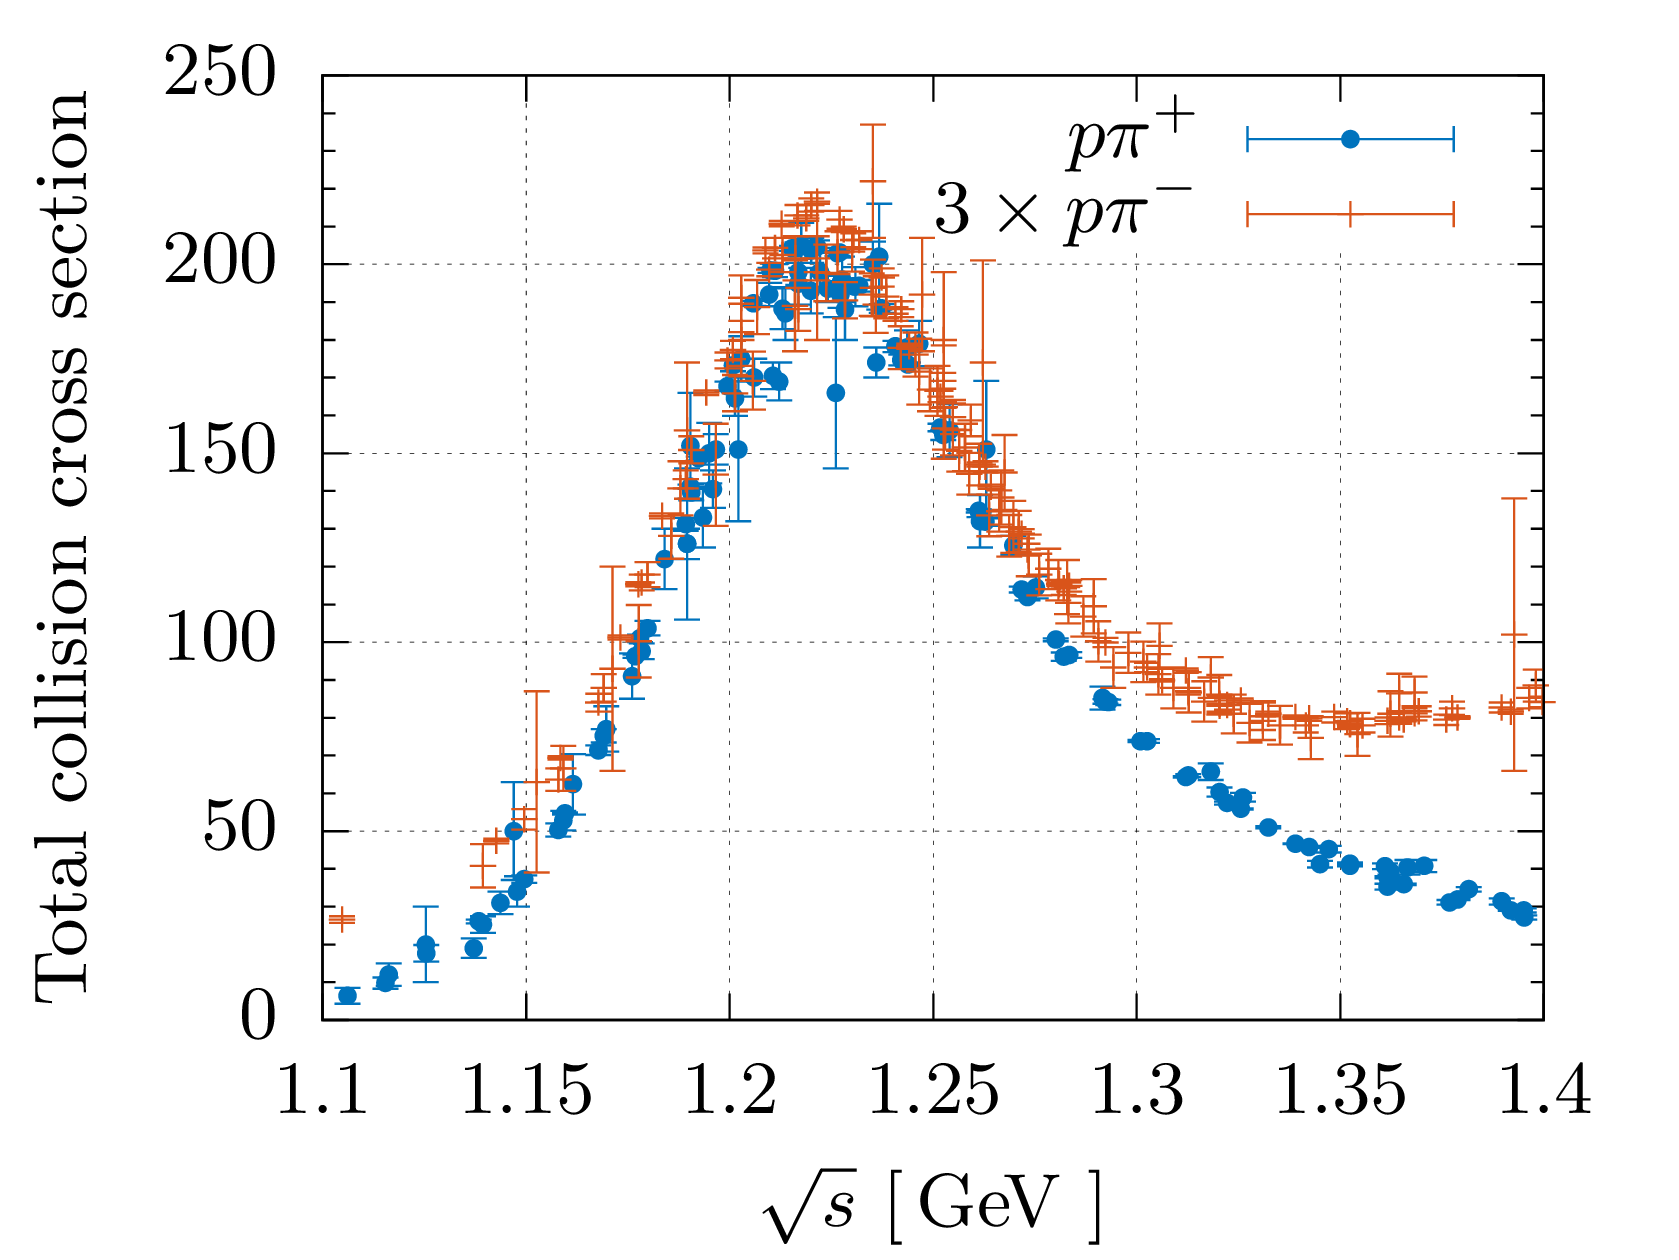
\includegraphics[scale=1.]{misc/pipp_xsec.png}
    \caption{Production rate of $\decay{\proton\pip}{\PDelta(1232)^{++}}$ and $\decay{\proton\pim}{\PDelta(1232)^0}$ with data taken from the Particle Data Group~\cite{ppiTotalSigma}. (Data files are courtesy of the COMPAS Group, IHEP, Protvino, Russia). Isospin conservation predicts an exact ratio of $3$ which is in good agreement with the measurements shown above (note the scaling of the $\proton\pim$ data).}
    \label{fig:ppiTotalSigma}
\end{figure}

An interesting case of isospin violation in strong decays is the decay $\decay{\Peta}{3 \pion}$. This strong decay of a $I^G \left( J^{PC} \right) = 0^+ \left( 0^{-+} \right)$ state into $1^- \left( 0^{-(+)} \right)$ states is forbidden by $G$-parity.
Since $G$-parity is a combination of isospin and $C$-parity and the latter is conserved, this decay indeed violates isospin symmetry.
Interestingly, $\decay{\Peta}{2 \pion}$ decays are forbidden by $C$-parity which makes the $3 \pion$ decays, albeit (approximately) forbidden, the dominant decay modes\footnote{This also explains the exceptionally narrow width of $\Peta$.}~\cite{etaDecays,etaTopippim,etaTopizpiz}
\begin{align*}
    \BR\left(\decay{\Peta}{\pip \pim \piz}\right) &= 22.6 \pm 0.5\,\% \,,\\
    \BR\left(\decay{\Peta}{\piz \piz \piz}\right) &= 34.0 \pm 0.8\,\% \,,\\
    \BR\left(\decay{\Peta}{\pip \pim}\right) &< 1.3 \times 10^{-5} \quad (\text{CL} = 90\%) \,,\\
    \BR\left(\decay{\Peta}{\piz \piz}\right) &< 3.5 \times 10^{-4} \quad (\text{CL} = 90\%) \,,
\end{align*}
and the branching fractions similar to the (isospin violating) electro-magnetic decay $\decay{\Peta}{\gamma\gamma}$~\cite{etaDecays}
\begin{equation*}
    \BR\left(\decay{\Peta}{\gamma\gamma}\right) = 38.5 \pm 0.5\,\% \,.
\end{equation*}
These measurements shine light onto the quantitative power of the isospin argument by showing, that strong, isospin forbidden decays are on the same level as QED transitions ($\mathcal{O}(\alpha^2)$ in this case).
In general, isospin breaking effects can be large in electro-weak decays but are suppressed when strong decays can contribute.
Furthermore, the suppression of isospin violation is considered largely independent of the momentum transfer ($Q$-value), \ie{}, isospin mixes two mass eigenstates, for example
$$\decay{\Lb}{\jpsi \left( \cos(\theta) \Lz + \sin(\theta) \Sigma^0 \right)},$$ 
where the mixing angle $\theta$ is largely independent of the momentum transfer~\cite{privcomGinoIsidori} and thus allows inferring the isospin suppression between decays with different $Q$-values.

\section{\texorpdfstring{\decay{\Sz}{\Lz\Pgamma}}{Σ → Λγ} Background}
\Lz and \Sigmares baryons are part of the baryon octet.
The former is an isospin singlet and the latter three resonances \Sm, \Sz, and \Sp form an isospin triplet.
The quantum numbers of the \Lz and the \Sz baryons are identical, including the common valence quarks (\uquark \dquark \squark), except for the isospin which separates the former as a singlet and the latter as part of the triplet.
The \Sz baryon can thus decay fast without quark transitions into the singlet state \Lz via emission of a soft photon.
Transitions between the \Sz and \Lz via strong interaction are forbidden due to the small isospin splitting, $m(\Sz) - m(\Lz) = 76.959(23)\mevcc$~\cite{pdg}, which is lighter than any meson mass.
Other decay channels besides \decay{\Sz}{\Lz\Pgamma} are $\BR(\decay{\Sz}{\Lz\Pgamma\Pgamma})<3\,\%$ (experimentally measured at a 90\,\% CL) and $\BR(\decay{\Sz}{\Lz\ep\en})= \num{5e-3}$ (theoretical \QED calculation)~\cite{SzToLzgg,SzToLzee}.

Due to the small isospin splitting, the photon of the radiative transition will almost always escape undetected at \lhcb and is therefore not included in the reconstruction step of the present analysis which makes the \Sz resonance a partially reconstructed background in most analyses with intermediate \Lz baryons.

\subsection{Limitations of \texorpdfstring{na\"ive \grpsutw{}}{naive SU(2)} Arguments}
Since both, \Lz and \Sz share the same valence quarks, the decision which of both actually hadronizes in decays is imposed by \QCD.
The production of \Lz and \Sz baryons in \QCD was studied at lepton colliders, \eg{}, by the \gls{besiii} collaboration in \jpsi and \psitwos decays \cite{LzSzProd}.
The results of Ref.~\cite{LzSzProd} are summarized in Tab.~\ref{tab:besiiiJpsiToLzLz}.

\begin{table}[htbp]
    \centering
    \caption{Results for branching fractions \BR of \Lz and \Sz production in charmonia decays taken from Ref.~\cite{LzSzProd}. Statistical and systematic uncertainties are added in quadrature. Additionally, we calculate the ratio of \Sz and \Lz branching fractions, based on the published results of Ref.~\cite{LzSzProd} and assign uncertainties obtained from linear error propagation while ignoring correlations.}
    \label{tab:besiiiJpsiToLzLz}
    \begin{tabular}{l%
                    S[separate-uncertainty=true,table-format=2.2(3)]%
                    c}
        \toprule
        Channel & {\BR~($\times 10^{-4}$)} & {Ratio} \\
        \midrule
        \decay{\jpsi}{\Lz\Lbar} & 19.43 \pm 0.33 & \multirow{2}{*}{\num{0.599 \pm 0.016}} \\
        \decay{\jpsi}{\Sz\Szbar} & 11.64 \pm 0.23 \\
        \decay{\psitwos}{\Lz\Lbar} & 3.97 \pm 0.12 & \multirow{2}{*}{\num{0.615 \pm 0.033}} \\
        \decay{\psitwos}{\Sz\Szbar} & 2.44 \pm 0.11 \\
        \bottomrule
    \end{tabular}
\end{table}

In the case of \Lz and \Sz production from charmonia resonances, hadrons are not only produced via QCD (OZI suppressed decays), but also via QED, \eg{}, \decay{\jpsi}{\decay{\gamma}{\Lz\Lbar}}.
Assuming isospin conservation for QCD, only the latter process gives rise to isospin breaking decays such as \decay{\jpsi}{\Lz \Szbar} which is a transition from an isospin singlet state $\ket{I=0, I_3=0}$ into $\ket{I=1,I_3=0}$.
Even though QED breaks isospin conservation, the single photon allows only one quark anti-quark pair to form a $I=0$ or $I=1$ state.
All other pairs still obey QCD and are thus isospin singlets, \ie{}, only final states of at most $\Delta I=1$ are possible.
The Clebsch-Gordan (CG) coefficients for a \Sz \Szbar pair are
$$\underbrace{\ket{1, 0}}_{\Sz} \otimes \underbrace{\ket{1, 0}}_{\Szbar} = \left\{ \frac{1}{3} \, \ket{0,0},\,\frac{2}{3} \, \ket{2, 0} \right\}.$$
Thus, even in the case of isospin violating $\Delta I=1$ processes, \Lz \Lbar and \Sz \Szbar pairs can only form a $I=0$ state.
Consequently, the branching ratio of \Lz \Lbar and \Sz \Szbar pairs should be governed by the corresponding CG coefficients, and thus be $1$ : $\sfrac{1}{3}$.
Experimentally, a ratio of $60\,\%$ is measured, thus pointing towards an additional isospin breaking contribution, such as final state interactions and possible corrections of a full \grpsuthree{} consideration.
%From a pure isospin consideration, a na\"ive expectation arises from Clebsch-Gordan (CG) coefficients and predicts a factor of $\sfrac{1}{3}$,
%$$\ket{1,0} \otimes \ket{1,0} = \left\{ \frac{1}{3} \, \ket{0,0},\,\frac{2}{3} \, \ket{2, 0} \right\},$$
%where $\ket{I, I_3}$ is an isospin configuration with magnitude $I$ and quantized projection $I_3$.
%Experimentally, however, a ratio of $60\,\%$ is measured, thus hinting towards an enhancement of \Sz resonances w.r.t.\ \Lz beyond angular momentum coupling effects.

When created in (OZI suppressed) strong decays, the initial isospin state of the \uquark-, \dquark- and \squark-quarks is well known due to the isospin conservation of \QCD, whereas the situation is more complicated in weak decays, since isospin conservation is not guaranteed anymore and thus the initial isospin state of the quarks is typically unknown.
\decay{\kaon}{\pion\pion} decays have a long history of revealing counter intuitive selection rules between different isospin states, \ie{}, the amplitudes of \decay{\KS}{\piz\piz}, \decay{\KS}{\pip\pim} and \decay{\Kp}{\pip\piz} can be used to unfold amplitudes corresponding to isospin states $I=0$ and $I=2$.\footnote{The $I=1$ final state is unreachable for pairs of pions due to their bosonic nature, \ie{}, bosons are described by symmetric wave functions, whereas combinations of odd angular momentum $L$ or odd isospin $I$ quantum numbers are antisymmetric. Hence $L$ and $I$ must either be both odd or both even. For kaon decays, $L=0$ and therefore $I$ can have only even values.}
Experimentally, the ratio of the amplitudes for $I=0$ and $I=2$ is measured to be larger than expected from the CG coefficients, thus hinting towards a suppression of large isospins beyond a na\"ive angular momentum coupling description.
In this particular case, this deviation is known as the so-called $\Delta I=\sfrac{1}{2}$ rule for kaons and is well described in theory, for example in the framework of chiral perturbation theory~\cite{DeltaIRule}.

%\subsection{From Emails with Sheldon}
%Gino Isidori / Jon Rosner: However, isospin is broken also in strong interactions by the quark masses. It is a small effect, but non zero (indeed we have \decay{\Peta}{\pion \pion \pion}, \Prho-\Pomega mixing...). So, I expect  \decay{\Lb}{\jpsi\Sz} to occur at a significantly lower rate than \decay{\Lb}{\jpsi \Lz}, but to be there. Actually the $m(\uquark)-m(\dquark)$ mass difference corresponds indeed to a $\Delta I = 1$ operator.
%
%Zoltan Ligeti: I do not think about isospin violation in terms of these Feynman diagrams.  The ($\bquark \cquarkbar \cquark \squarkbar$) part of the weak Hamiltonian (from integrating out the \W), pictured in the diagram you sent me, will generate both decays, but the \Sz final state should be substantially suppressed compared to the \Lz final state, as the former is isospin violating. I think it is definitely worth measuring!  We have very little data on how significant a suppression corresponds to isospin violation in these type of decays, it can teach us about QCD, SCET, factorization, etc.
%
%Roland: \decay{\Peta}{\pion \pion \pion}: hier schlaegt wieder mal die G-Paritaet zu: \Peta hat +, 3 Pionen haben -. Und G-Paritaet beruht auf C-Paritaet und Isospin. Da wir annehmen, dass C erhalten ist, ist der Isospin verletzt. Das ist in der Tat ein interessantes Beispiel, da vermutlich die elmgn. WW. (die Isospin verletzt) nicht ausreicht. Meines Wissens spielt dabei eine Rolle, dass die pis und das \Peta relativ leicht sind, sodass die kleine MAssendifferenz \dquark-\uquark ein messbaren $\Delta I$ Uebergang bewirken kann. Isospinverletzung gibt es (im Prinzip in grossem Stil) in der schwachen WW und der elmgn. WW.  Beide sind aber viel schwaecher als die starke WW, weshalb Isospinverletzung meist ein kleiner Effekt ist, wenn die starke WW auch beitragen kann. Darueberhinaus verletzen die Yukawa-Kopplungen des Higgs auch den Isospin, d.h. u und d haben verschiedene Massen.
%Das spielt immer dann eine Rolle, wenn die Q-Werte klein sind.

\subsection{Background Contamination by \texorpdfstring{\decay{\Sz}{\Lz\Pgamma}}{Σ → Λγ} at \lhcb}
Since the soft photon in \decay{\Sz}{\Lz\Pgamma} cannot be reconstructed at \lhcb, most analysis with intermediate \Lz resonances will be contaminated with the partially reconstructed background events of \Sz decays which are irreducible.

For example, this is the case in the charmless two-body decay \decay{\Bu}{\proton\Lbar}, analyzed at \lhcb~\cite{BuTopLzb}.
Penguin contributions with a \decay{\bquarkbar}{\squarkbar} loop are expected to dominate, but tree-level and annihilation diagrams also contribute.
Electro-weak penguins and tree diagrams create a \uquark\uquarkbar or \dquark\dquarkbar pair that couples with the spectator quark either into an isospin $I=\sfrac{1}{2}$ or $I=\sfrac{3}{2}$ state, corresponding to $\Delta I = 0$ and $\Delta I = 1$, respectively.
The other \quark\quarkbar pair is created from the QCD vacuum and thus does not change the total isospin.
In case of the annihilation diagram and gluon penguins, two \quark\quarkbar pairs are created form the QCD vacuum and only $\Delta I=0$ is possible.

%Here, the \dquark \dquarkbar vacuum pair is an isospin singlet, whereas the quarks from the quark transition \decay{\bquark}{\uquark \squark \uquarkbar} (tree or penguin diagram) and the spectator quark can form an isospin doublet and quadruplet state,
%\begin{equation}
%    \label{eq:BuTopLzbQuarks}
%    \underbrace{\ket{0, 0}}_{\text{vacuum}} \otimes \underbrace{\ket{\frac{1}{2}, +\frac{1}{2}} \otimes \ket{\frac{1}{2}, -\frac{1}{2}}}_{\bquarkbar \, \to \, \uquarkbar \, \squarkbar \uquark} \otimes \underbrace{\ket{\frac{1}{2}, +\frac{1}{2}}}_{\text{spectator}} = \left\{ \frac{2}{3} \, \ket{\frac{1}{2}, \frac{1}{2}},\, \frac{1}{3} \, \ket{\frac{3}{2}, \frac{1}{2}} \right\}.
%\end{equation}
The quark states can hadronize as either \proton\Lbar or \proton\Szbar, \ie{},
\begin{align*}
    \proton\Lbar &: \quad \ket{\frac{1}{2}, \frac{1}{2}} \otimes \ket{0, 0} = \ket{\frac{1}{2}, \frac{1}{2}} \,,\\
    \proton\Szbar &: \quad \ket{\frac{1}{2}, \frac{1}{2}} \otimes \ket{1, 0} = \left\{ \frac{1}{3} \, \ket{\frac{1}{2}, \frac{1}{2}},\, \frac{2}{3} \ket{\frac{3}{2}, \frac{1}{2}} \right\} \,.
\end{align*}
Inferring a suppression of $\Delta I=1$ from the $\Delta I=\sfrac{1}{2}$ selection rule for kaons, \Sz resonances would be suppressed by a factor of $\sfrac{1}{3}$. Vice-versa, if $\Delta I = 0$ would be suppressed, then electro-weak penguins and tree diagrams would induce an increase of \Sz hadronization.
The fit to recorded \decay{\Bu}{\proton\Lbar} events at \lhcb prefers the former option by finding $N(\decay{\Bu}{\proton\Szbar})$ being compatible with zero but $N(\decay{\Bu}{\proton\Lbar}) = 13.0^{+5.1}_{-4.3}$~\cite{BuTopLzb}.
We note, that the amount of available statistics in this channel is similar to \decay{\Lb}{\Dz\Lz} where we expect the very same suppression factor.
(Even without relying on \enquote{mysterious $\Delta I$ rule[s]}, \cf Ref.~\cite{DeltaIRule}.)

In Tab.~\ref{tab:SzInLbDecays} we show a selection of \Lb decays with an intermediate \Lz baryon together with the corresponding \Lz-\Sz asymmetry
\begin{equation}
    \label{eq:theory_lzszasym}
    a(\Lz : \Sz) := \frac{f(\Lz) - f(\Sz)}{f(\Lz) + f(\Sz)} \,,
\end{equation}
where $f(\Lz)$ and $f(\Sz)$ refer to the amounts of \Lz and \Sz, respectively.
An asymmetry of $-1$, $0$, $+1$ thus corresponds to a pure \Sz, balanced \Lz and \Sz, and pure \Lz decay, respectively.

For some of the decays listed in Tab.~\ref{tab:SzInLbDecays} \W-exchange diagrams are also possible (\eg{}, Ref.~\cite{wexchange}) which are often considered suppressed in the literature.
We note, that a strong suppression is only given for mesons due to the required spin alignment of the quark and anti-quark pair, but that this is not necessarily the case for baryons.

The decays $\decay{\Lb}{\Lz\Ph\Ph'}$, \decay{\Lb}{\Lz\Pphi} and \decay{\Lb}{\jpsi\Lz} were analyzed at \lhcb~\cite{LbToLzhh,LbToLzphi,LbToJpsiLz}, whereas the other decays are subject of the present analysis.
The ranges for the values of the \Lz-\Sz asymmetry arises from the yet unknown $\Delta I$ selection rules we mentioned above.
For example, the \uquark-quark produced via \W-exchange in the \decay{\Lb}{\Lz\Pphi} decay can either end within a $\ket{0, 0}$ or a $\ket{1, 0}$ state together with the spectator, corresponding to a \Lz-\Sz asymmetry of either $1$ or $-1$, respectively.
In the case of tree and penguin decays of the \Lb baryon, we can further constrain the possible combinations by observing, that the spectator diquark (\uquark \dquark) is an isospin singlet state $\ket{0, 0}$ which is, since not involved in the decay in leading order, conserved.
In decays via \W-exchange, this initial singlet state is broken, though, and the spectator quark can contribute in the subsequent isospin coupling.
\begin{table}[htbp]
    \centering
    \caption{Selection of \Lb decays with an intermediate \Lz baryon, primary quark transitions, and \Lz-\Sz asymmetry $a(\Lz:\Sz)$ as defined in Eq.~\eqref{eq:theory_lzszasym}. For decays via \W-exchange the spectator quark has to be included into the isospin coupling (flavor is shown in parentheses).}
    \label{tab:SzInLbDecays}
    \begin{tabular}{lllc}
        \toprule
        Channel & Quark transition && \Lz-\Sz asymmetry \\
        \midrule
        \decay{\Lb}{\Lz\pip\pim} & \decay{\bquark}{\uquark \squark \uquarkbar} & (tree \& penguin) & $\sfrac{1}{9} \ldots \sfrac{1}{3}$ \\
        & \decay{\bquark}{\squark \dquark \dquarkbar} & (penguin) & $\sfrac{1}{9} \ldots \sfrac{1}{3}$ \\
        & \decay{\bquark \uquark (\dquark)}{\uquark \squark (\dquark)} & (exchange) & $\sfrac{1}{9} \ldots \sfrac{1}{3}$ \\
        \midrule
        \decay{\Lb}{\Lz\Kp\pim} & \decay{\bquark}{\uquark \dquark \uquarkbar} & (tree \& penguin) & $-\sfrac{1}{6} \ldots \sfrac{1}{3}$ \\
        & \decay{\bquark}{\dquark \squark \squarkbar} & (penguin) & $\sfrac{1}{3}$ \\
        & \decay{\bquark \uquark (\dquark)}{\uquark \dquark (\dquark)} & (exchange) & $-\sfrac{1}{6} \ldots \sfrac{1}{3}$ \\
        \midrule
        \decay{\Lb}{\Lz\Kp\Km} & \decay{\bquark}{\squark \uquark \uquarkbar} & (tree \& penguin) & $0 \ldots \sfrac{1}{2}$ \\
        & \decay{\bquark}{\squark \squark \squarkbar} & (penguin) & $\sfrac{1}{2}$ \\
        & \decay{\bquark \uquark (\dquark)}{\uquark \squark (\dquark)} & (exchange) & $0 \ldots \sfrac{1}{2}$\\
        \midrule
        \decay{\Lb}{\Lz\Pphi} & \decay{\bquark}{\squark \squark \squarkbar} & (penguin) & $1$ \\
        & \decay{\bquark \uquark (\dquark)}{\uquark \squark (\dquark)} & (exchange) & $-1 \ldots 1$ \\
        \midrule
        \decay{\Lb}{\jpsi\Lz} & \decay{\bquark}{\cquark \cquarkbar \squark} & (tree \& penguin) & $1$ \\
        & \decay{\bquark \uquark (\dquark)}{\uquark \squark (\dquark)} & (exchange) & $-1 \ldots 1$ \\
        \midrule
        \decay{\Lb}{\Dz\Lz} & \decay{\bquark}{\cquark \uquarkbar \squark} & (tree) & $\sfrac{1}{2}$ \\
        & \decay{\bquark \uquark (\dquark)}{\cquark \squark (\dquark)} & (exchange) & $\sfrac{1}{2}$ \\
        \midrule
        \decay{\Lb}{\Dzb\Lz} & \decay{\bquark}{\uquark \squark \cquarkbar} & (tree) & $\sfrac{1}{2}$ \\
        \midrule
        \decay{\Xibz}{\Dz\Lz} & \decay{\bquark}{\cquark \dquark \uquarkbar} & (tree) & $-1 \ldots \sfrac{1}{2}$ \\
        & \decay{\bquark \uquark (\squark)}{\cquark \dquark (\squark)} & (exchange) & $\sfrac{1}{2}$ \\
        \midrule
        \decay{\Xibz}{\Dzb\Lz} & \decay{\bquark}{\uquark \dquark \cquarkbar} & (tree) & $-1 \ldots \sfrac{1}{2}$ \\
        \bottomrule
    \end{tabular}
\end{table}

Most interesting for the present analysis is the ratio of the absolute amount of reconstructed decays with intermediate \Lz and \Sz in order to estimate the background contamination of \decay{\Lb}{\Dz\Sz} in \decay{\Lb}{\Dz\Lz}.
Unfortunately, there are a couple of caveats with na\"ively interpreting the yields of the fitted modes.
For example in the analysis of $\decay{\Lb}{\Lz\Ph\Ph'}$ decays, the authors could only account for partially reconstructed background components with a missing soft photon in general, due to the lack of experimental data of further \Lb background candidates~\cite{LbToLzhh}.
Contributions of \decay{\Sz}{\Lz\Pgamma} are, however, most physically motivated, but only one reasonable instance.
Unfortunately, the partially reconstructed background \decay{\Sz}{\Lz\Pgamma} peak in roughly the same place as the cross-feed contribution, which is quite well understood, but as the corresponding signal yields are small, this results in a reasonable uncertainty on which contributions are which.
Additionally, the same problem occurs in the \decay{\Lb}{\Lc\Ph} control mode where the \Lc can either decay into \Lz \pip or \Sz \pip.
Both of these amplitudes are measured by the \gls{besiii} collaboration and found to be significantly greater than zero~\cite{LcBR} and thus pollute the interpretation of the fitted yields as the true charmless decays, without \Lc component.
Luckily for the present analysis, this effect is most pronounced in the \Lz\pip\pim final state (\cf{}~Chap.~\ref{chap:bkgs}).
The branching fractions for corresponding modes with kaons are considerably more suppressed.

\subsection{Summary}
Isospin (non-)conservation is helpful for deciding whether or not a decay is suppressed.
Finding exact branching ratios, though, can be error prone as we saw in the case of \Lz\Lbar vs.\ \Sz\Szbar production or due to yet unknown $\Delta I$ selection rules.
However, in the case of \decay{\Lb}{\Dz\Lz} the situation is much easier and we do not expect large corrections neither to the tree, nor to the \W-exchange diagram. 

Regarding the available statistics, we will not be able to constrain or extract the relative branching ratio but we find it noteworthy to mention, that the \Sz modes are of great interest for future experiments for at least two reasons:
First, for the same reasons \CP violation is expected in \decay{\Lb}{\PD\Lz}, it is also expected for \decay{\Lb}{\PD\Sz} with different strong phases.
Secondly, \grpsuthree{} considerations yield relations among the amplitudes of \decay{\Lb}{\Dz\PX} and \decay{\Xibz}{\Dz\PX} decays~\cite{privyuval}:
\begin{align*}
    1 - \sqrt{3} \frac{\mathcal{A}(\decay{\Lb}{\Dz\Lz})}{\mathcal{A}(\decay{\Lb}{\Dz\Sz})} + \sqrt{2} \frac{\mathcal{A}(\decay{\Xibz}{\Dz\Xiz})}{\mathcal{A}(\decay{\Lb}{\Dz\Sz})} &= 0 \,, \\
    1 + \sqrt{3} \frac{\mathcal{A}(\decay{\Lb}{\Dz\Lz})}{\mathcal{A}(\decay{\Lb}{\Dz\Sz})} - 2 \frac{\lambda_s}{\lambda_d} \frac{\mathcal{A}(\decay{\Xibz}{\Dz\Sz})}{\mathcal{A}(\decay{\Lb}{\Dz\Sz})} &= 0 \,, \\
    1 - 2 \frac{\lambda_d}{\lambda_s} \frac{\mathcal{A}(\decay{\Lb}{\Dz\Sz})}{\mathcal{A}(\decay{\Xibz}{\Dz\Sz})} + \sqrt{3} \frac{\mathcal{A}(\decay{\Xibz}{\Dz\Lz})}{\mathcal{A}(\decay{\Xibz}{\Dz\Sz})} &= 0 \,, \\
    1 - \sqrt{3} \frac{\mathcal{A}(\decay{\Lb}{\Dz\Lz})}{\mathcal{A}(\decay{\Lb}{\Dz\Sz})} + \sqrt{2} \frac{\lambda_s}{\lambda_d} \frac{\mathcal{A}(\decay{\Lb}{\Dz\neutron})}{\mathcal{A}(\decay{\Lb}{\Dz\Sz})} &= 0 \,,
\end{align*}
with
\begin{align*}
    \lambda_d &:= \Vuds\Vcb \,, \\
    \lambda_s &:= \Vuss\Vcb \,.
\end{align*}
These should be tested and used to constrain decays that are unavailable for current experiments such as \decay{\Lb}{\Dz\neutron}.

\section{\texorpdfstring{\CP Violation in \bquark-Baryon Decays}{CP Violation in b-Baryon Decays}}
\label{sec:lbcpv}
\CP violation is an interference effect and originates from the complex phases of the \gls{ckm} matrix.
In order to get a measurable physical quantity in amplitudes the given observable has to come from the superposition of two (or more) decay modes that contribute a \CP even and a \CP odd term (\gls{ckm} phases are \CP odd) such that the interference term does not cancel in the magnitude.
In general, such decay modes are categorized into three classes, direct \CP violation, \CP violation in mixing, and \CP violation in interference of mixing and decays (\cf{} any good text book about flavor physics for more details).
Mesons offer a rich laboratory for measuring \CP violation among all three classes, \eg{}, Refs.~\cite{bsmixing,BsTohh_timecpv}.
In baryonic systems, and in particular in decays of \bquark-baryons such as the \Lb or \Xibz baryon, there can be no mixing due to conservation of baryon number and therefore no indirect \CP violation.
Studies of direct \CP violations are often limited to measuring asymmetries, since the \CP even phases have to be taken from theory which makes the result model dependent and typically come with large uncertainties~\cite{LbCPVAsym1,LbCPVAsym2}.
Lately, two methods have been proposed to overcome this issue~\cite{CPVbeautiful,brLbToDzLz_pred}.
They reinterpret methods original proposed by Atwood, Dunietz and Soni~\cite{ads1,ads2}, referred to as \gls{ads}, and a method first proposed by Gronau, London and Wyler~\cite{glw1,glw2}, referred to as \gls{glw}, that are already successfully carried out in decays of mesons~\cite{BdToDzKstar}, now for decays of baryons.
As proposed, these methods allow a clean extraction of the \gls{ckm} phase $\gamma$ in a model independent way\footnote{In particular the proposed modes do not suffer from penguin pollution.} and at the same time neither require tagging nor time-dependence.
In particular, in the \gls{ads} method $\gamma$ can be extracted by the study of the six decays \decay{\Lb}{\Dz\Lz}, \decay{\Lb}{\Dzb\Lz}, $\decay{\Lb}{\PD_{\CP}\Lz}$, and the respective \Lbbar modes, where
\begin{equation*}
    \PD_{\CP} \equiv
    \begin{dcases}
        \frac{\ket{\Dz} + \ket{\Dzb}}{\sqrt{2}} & \text{if \CP-even modes are considered,} \\
        \frac{\ket{\Dz} - \ket{\Dzb}}{\sqrt{2}} & \text{else.}
    \end{dcases}
\end{equation*}
Key to the present analysis is the idea, to enhance the \CP violating contribution by reconstructing $\decay{\Lb}{[\Kp\pim]_{\PD}\Lz}$ which compensates the suppression of \decay{\Lb}{\Dzb\Lz} by favoring the Cabibbo (doubly) suppressed \decay{\Dz}{\Kp\pim} mode in the \decay{\Lb}{\Dz\Lz} decay (\cf{}~Fig.~\ref{fig:decaysLbToDzLz}).
\begin{figure}
    \centering
    \begin{subfigure}{.49\textwidth}
        \centering
        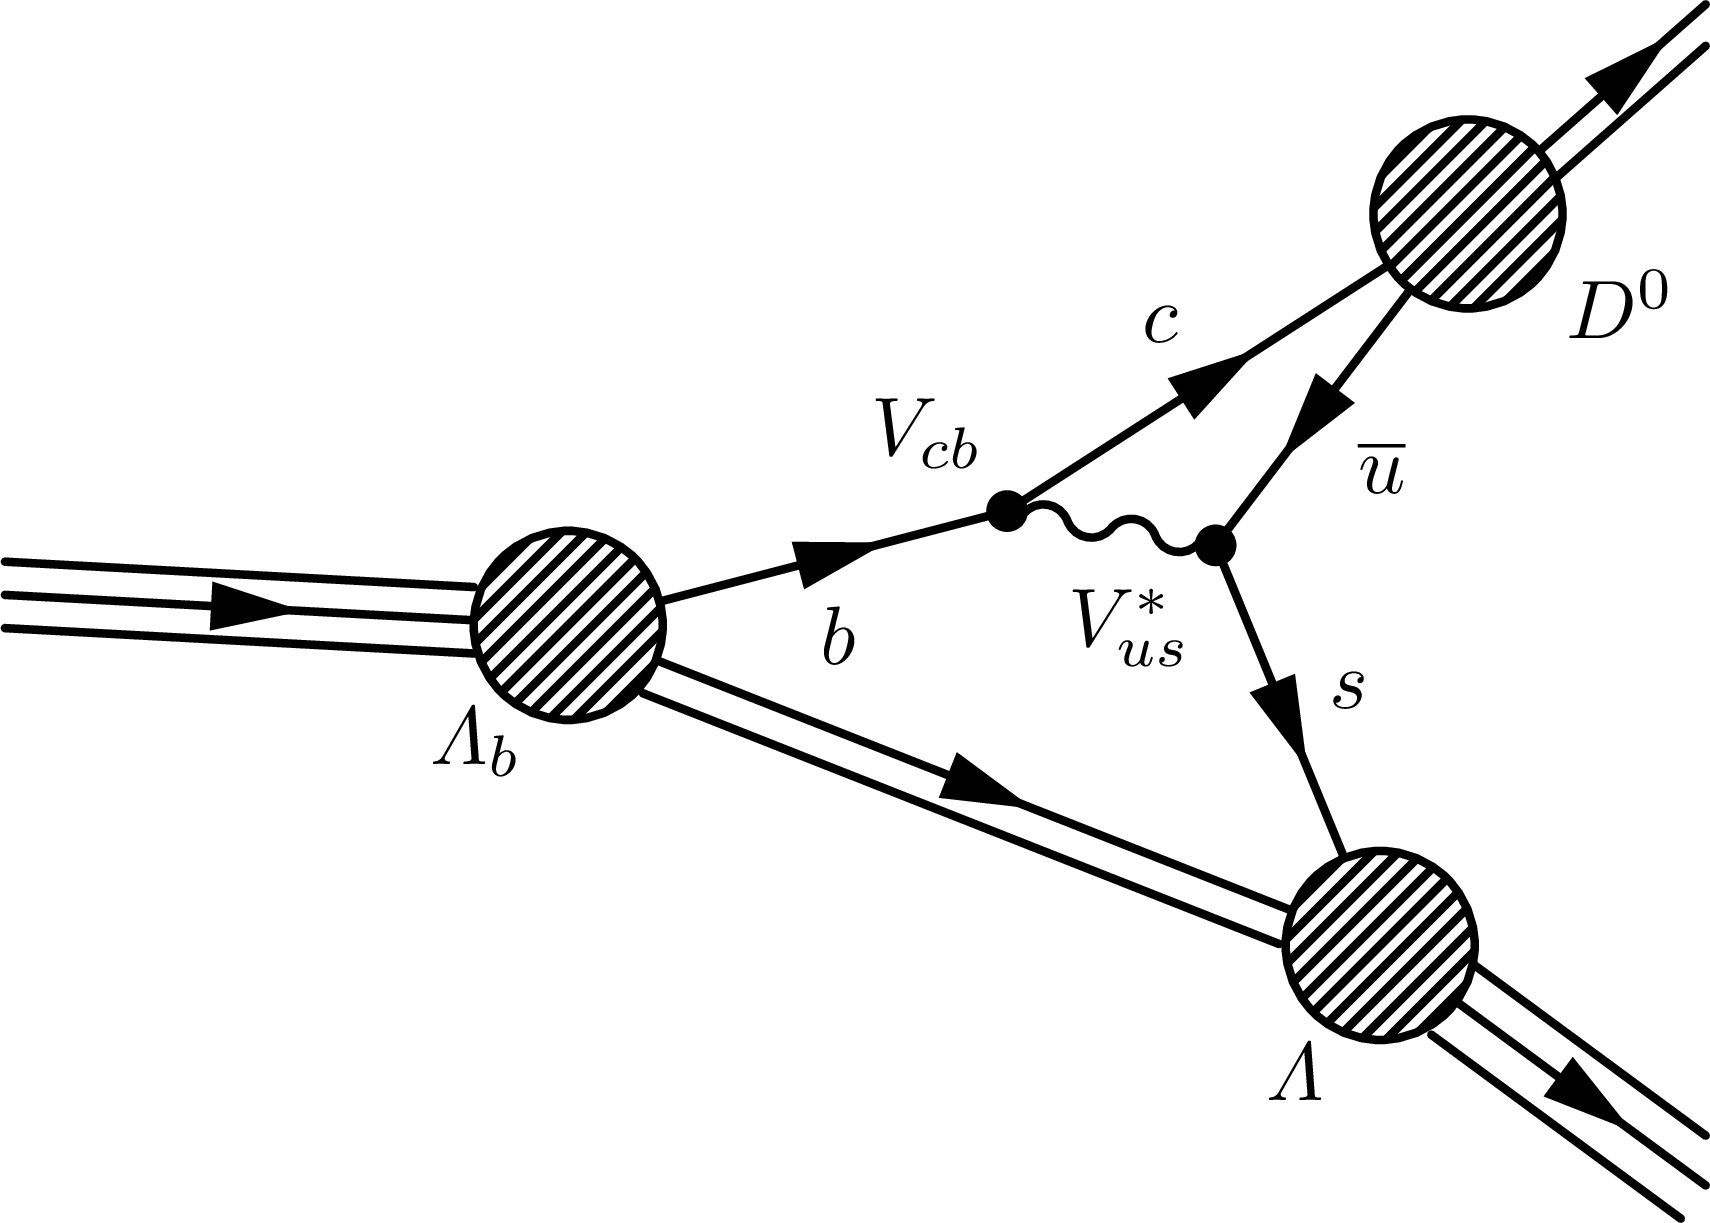
\includegraphics[scale=.1]{misc/decayLb2DzLz.png}
        \caption{\decay{\Lb}{\Dz\Lz}}
    \end{subfigure}
    \begin{subfigure}{.49\textwidth}
        \centering
        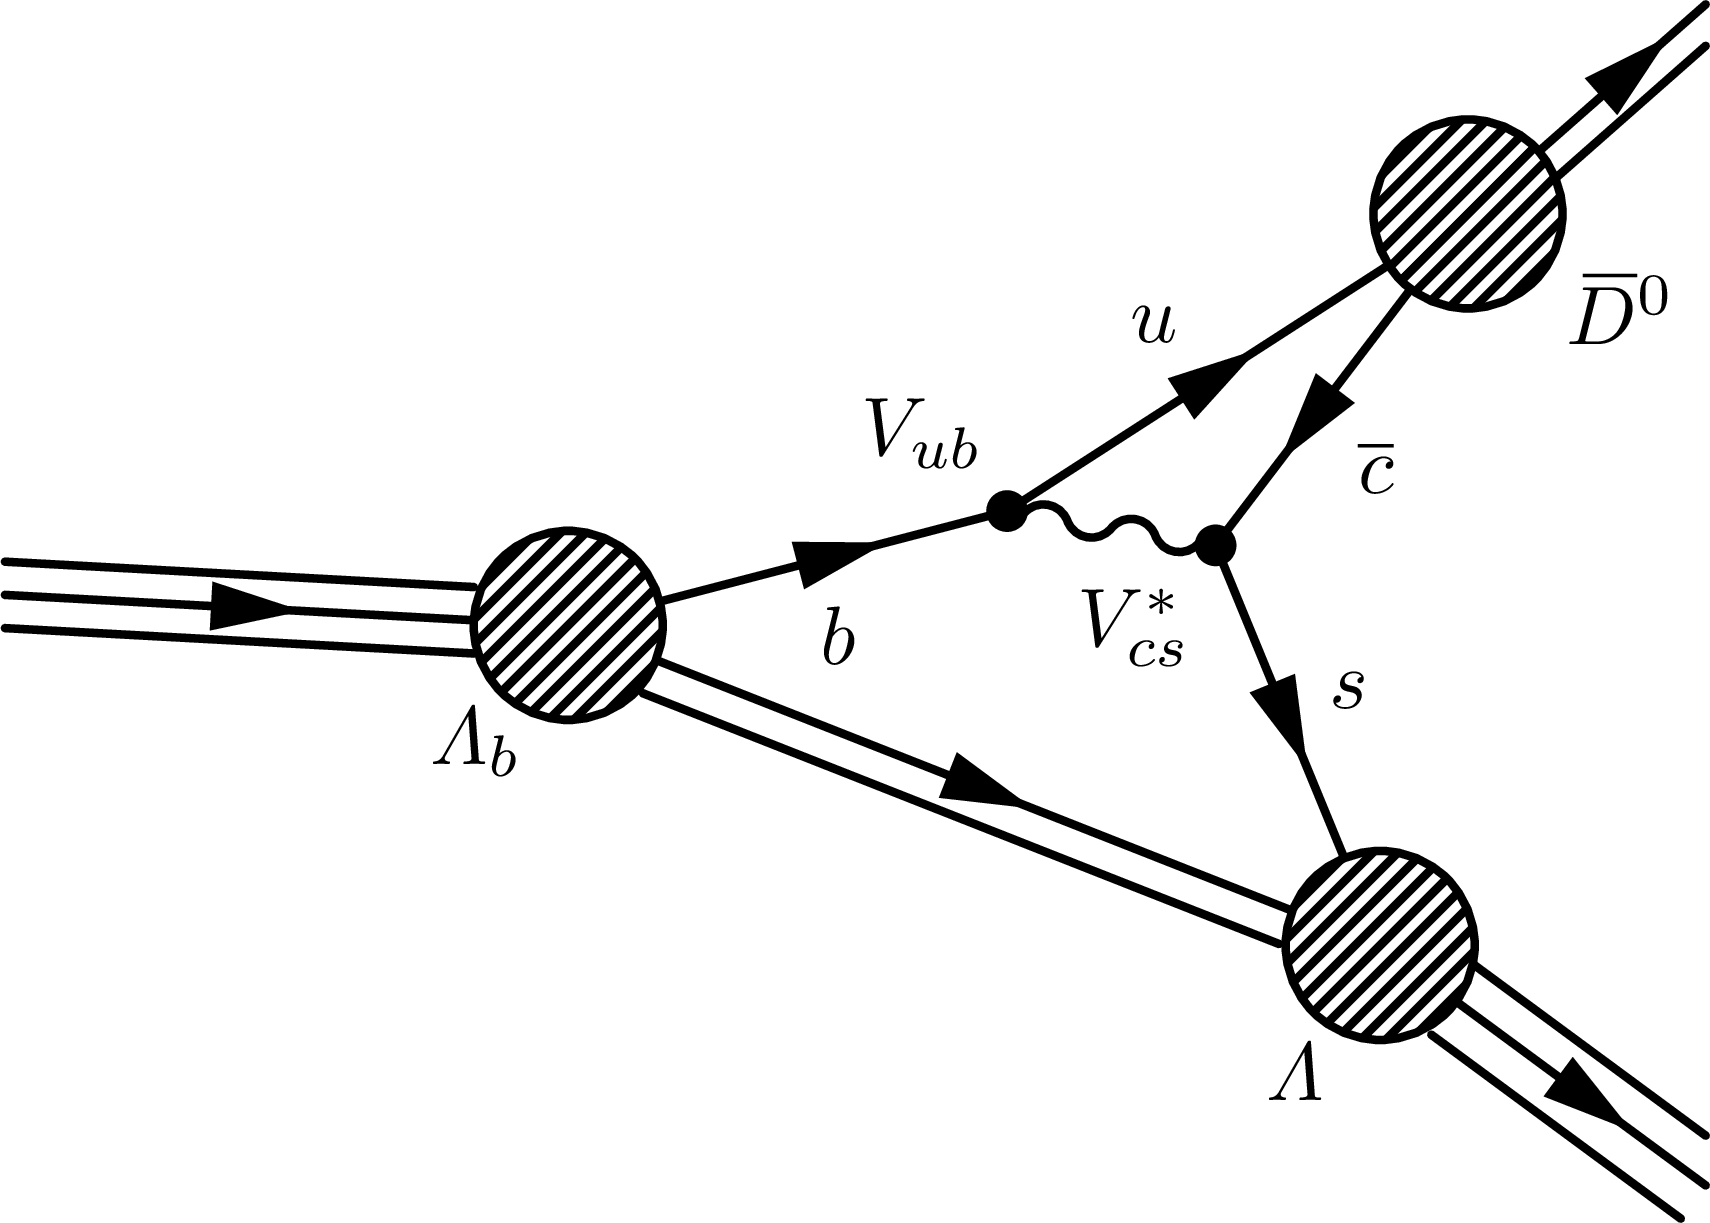
\includegraphics[scale=.1]{misc/decayLb2DzbLz.png}
        \caption{\decay{\Lb}{\Dzb\Lz}}
    \end{subfigure}
    \caption{Feynman diagrams of the decays \decay{\Lb}{\Dz\Lz} and \decay{\Lb}{\Dzb\Lz}. The latter decay is strongly suppressed w.r.t.\ to the former due to the \decay{\bquark}{\uquark} transition. The suppression can be reduced by reconstructing \decay{\PD}{\Kp\pim} which is Cabibbo doubly suppressed for the former but Cabibbo favored for the latter.}
    \label{fig:decaysLbToDzLz}
\end{figure}
Further, the statistics of the studies can be enriched by also including the four-body modes $\decay{\PD}{\Kpm\pimp\pip\pim}$.
Similarly, the same technique is applicable to other two-body decays, such as $\decay{\Xires_\bquark^{0/-}}{\PD\Xires^{0/-}}$ and $\decay{\Omegab}{\PD\Omegares^0}$ but also to the various backgrounds of the present analysis (\cf{}~Chap.~\ref{chap:bkgs}) and also three-body decays such as \decay{\Lb}{\Dz\proton\Km} or \decay{\Lb}{\Lz\pip\pim}~\cite{cpvinLbToLzpipi}. (The latter is also well suited for measurement of $T$ violation with triple products~\cite{tvinLbToLzpipi}.)
We note further that in all these modes, the \CP violation is encoded in the entire decay chain, do not rely on \CP violation in the \PD meson system and thus genuinely leverages the observation of \CP violation in baryon decays. 
The same holds for the cited \gls{glw} method where the \Dz and \Dzb are reconstructed in \CP eigenstates \Kp\Km and \pip\pim.

In contrast to the two-body decay modes, the three-body decay modes have to be studied in Dalitz plots that require a meticulous description of the various background and resonance contributions.
%In particular, the many resonances in \decay{\Lb}{\Dz\proton\Km} studies require thorough analyses~\cite{hviemann}.
On the contrary, two-body decays come with significant smaller sample sizes at \lhcb, due to the lower branching fraction, and reconstruction and trigger inefficiencies of the long living \Lz baryons, but offer a much easier to analyze decay topology.
Since none of the \decay{\Lb}{\PD\Lz} decays have been observed at the time of writing, the main focus of the present analysis is to establish a branching ratio for \decay{\Lb}{\Dz\Lz} by reconstructing \decay{\Dz}{\Km\pip} (and thus neglecting Cabibbo doubly suppressed contributions from \decay{\Lb}{\Dzb\Lz}).
We find the available dataset also sensitive to the decay \decay{\Xibz}{\Dz\Lz} which is on its own a candidate for measuring \CP violation.
We note that a \CP violation study of the \Xibz decay using the \gls{ads} method does not suffer from a contamination of charmless backgrounds\footnote{Due to the absence of \decay{\Xibz}{\Lz\Kp\pim} decays, \cf{}~Sec.~\ref{sec:bkgs_refl}.} as it is the case for \CP violation studies of the corresponding \Lb decay, whereas the expected amount \CP violation is much lower.
